\documentclass{article}

\usepackage{url,graphicx,tabularx,array,geometry, hyperref}
\usepackage{listings}
\usepackage{fullpage}
\usepackage{fancyvrb}
\usepackage{framed}
\usepackage{lastpage}
\usepackage{fancyhdr}
\usepackage{float}
\usepackage[hyperref=true, natbib=true, style=numeric, backend=bibtex]{biblatex}
\bibliography{references.bib}

\renewcommand{\headrulewidth}{0pt}
\setcounter{secnumdepth}{0}

\setlength{\parskip}{1ex} %--skip lines between paragraphs
\setlength{\parindent}{0pt} %--don't indent paragraphs
\setlength{\headheight}{15.2pt}

\pagestyle{fancy}

\renewcommand{\headrulewidth}{0pt}
\lhead{  }
\lfoot{Lab 1: TCP Congestion Control}
\rfoot{page \thepage\ of \pageref{LastPage}}

\renewcommand{\familydefault}{\sfdefault}
\begin{document}

\begin{titlepage}
\begin{center}
\textsc{\huge \bfseries Advanced Networking 2018}\\[1.5cm]
\textsc{\large Lab \#1: TCP Congestion Control}\\[1.5cm]
\textsc{\huge Report}\\[1.5cm]
\textsc{\huge \bfseries GROUP: 1}\\[1.5cm]
\textsc{\large{\textbf{Authors:}\\ Rick van Gorp, rick.vangorp@os3.nl\\ Luc Gommans, os3@lucgommans.nl}}

\textsc{\large University of Amsterdam}
\end{center}
\end{titlepage}

\subsection{Q1.1 Plot a graph showing CWND versus time from 0.0s to 100.0s.}

\begin{figure}[H]
	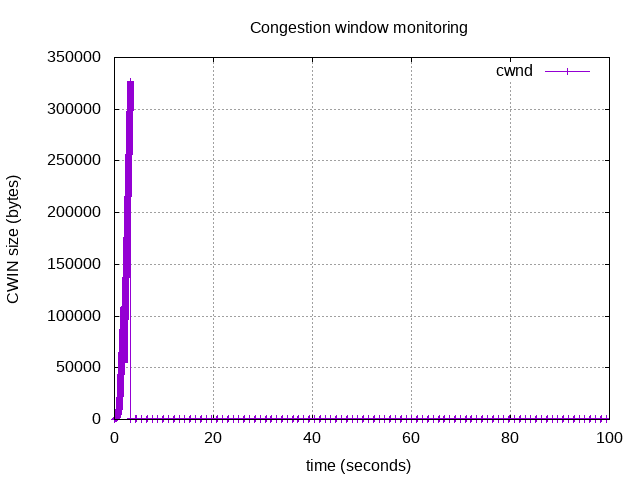
\includegraphics{lab1-group1-task1-question1.png}
	%\label{fig:dinges}
	\caption{T1Q1 CWND from 0 to 100 seconds}
\end{figure}



\subsection{Q1.2 Plot a graph showing SSTH versus time from 0.0s to 100.0s.}

\begin{figure}[H]
	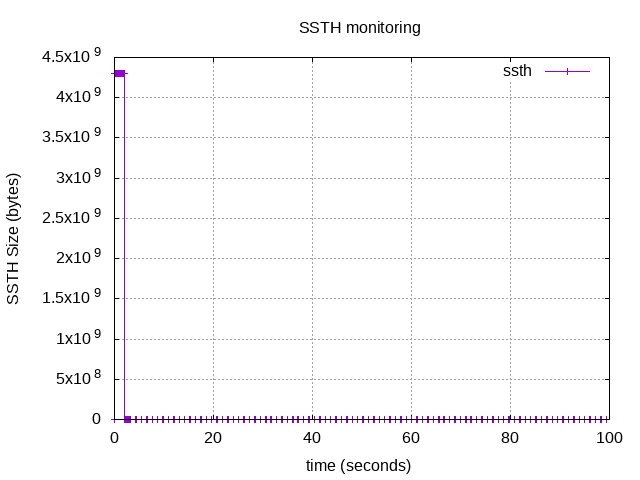
\includegraphics{lab1-group1-task1-question2.png}
	%\label{fig:dinges}
	\caption{T1Q2 SSTH from 0 to 100 seconds}
\end{figure}


\subsection{Q1.3 Find the points where the slow-start, congestion-avoidance, fast retransmit/fast recovery states begin.}
Table \ref{table:results1} shows the points where the slow-start, congestion-avoidance and fast recovery states begin.
The results are based on the reno datafiles generated in the vagrant boxes and the states described in the slidedeck of lecture 1.
We found the slow-start state starts at 0 seconds and is followed by the fast recovery state as $ssthresh$ halves and $cwnd$ becomes 3 higher than $ssthresh$.
After the fast recovery state we see that the algorithm goes to the slow start state again and then, after some time $cwnd$ exceeds $ssthresh$. From here the transition from slow start to congestion-avoidance occured.

\begin{table}[H]
\center
\caption{Points of state transitions NewReno algorithm}
\label{table:results1}
\begin{tabular}{|c|p{25mm}|p{20mm}|c|c|}
\hline Time (s)    & Current CWND (bytes)    & New CWND (bytes)    & New State             & Event            \\
\hline 0.00000     & 0                       & 340                 & slow-start            & start            \\ 
\hline 1.93189     & 109 480                 & 55 590              & fast-recovery         & dupACKcount==3   \\ 
\hline 3.26916     & 326 570                 & 340                 & slow-start            & timeout          \\ 
\hline 3.30286     & 340                     & 680                 & congestion-avoidance  & cwnd$>=$ssthtresh  \\ 
\hline  
\end{tabular} 
\end{table}


\subsection{Q1.4 Plot a graph showing CWND versus time from 0.0s to 100.0s.}

\begin{figure}[H]
	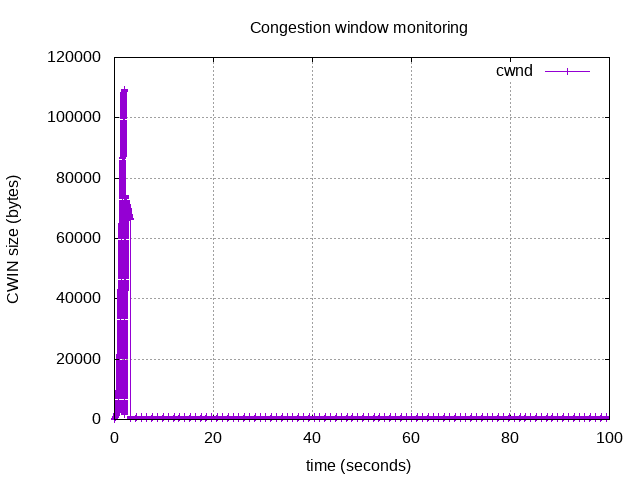
\includegraphics{lab1-group1-task1-question4.png}
	%\label{fig:dinges}
	\caption{T1Q4 CWND from 0 to 100 seconds}
\end{figure}


\subsection{Q1.5 Plot a graph showing SSTH versus time from 0.0s to 100.0s.}

\begin{figure}[H]
	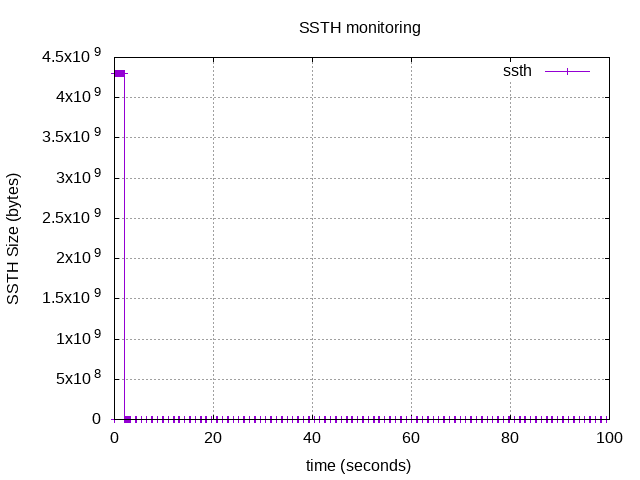
\includegraphics{lab1-group1-task1-question5.png}
	%\label{fig:dinges}
	\caption{T1Q5 SSTH from 0 to 100 seconds}
\end{figure}


\subsection{Q1.6 Find the points where the slow-start, congestion-avoidance, fast retransmit/fast recovery states begin.}

\begin{table}[H]
\center
\caption{Points of state transitions WestWood algorithm}
\label{table:results2}
\begin{tabular}{|c|p{25mm}|p{20mm}|c|c|}
\hline Time (s)    & Current CWND (bytes)    & New CWND (bytes)    & New State             & Event            \\
\hline 0.00000     & 0                       & 340                 & slow-start            & start            \\ 
\hline 1.93189     & 109480                  & 1700                & fast-recovery         & dupACKcount==3   \\ 
\hline 2.26758     & 74 120                  & 73 100              & congestion avoidance  & New ACK  \\ 
\hline 3.19086     & 66 640                  & 340                 & fast-recovery         & dupACKcount==3 \\ 
\hline  
\end{tabular} 
\end{table}



The strange part of this graph is the section between 2.2 and 3.3 seconds,
where the congestion window slowly decreases. We could initially not attribute
it to the state machine, nor could we find a paper which described this
behavior. Looking in the source code of NS3, we believe the following line
is responsible for it:

\texttt{m\_currentBW = m\_ackedSegments * tcb->m\_segmentSize / rtt.GetSeconds ();}

Because the estimated RTT increases, the current bandwidth estimate decreases
from 11 301 to 3081. All other variables in the source code appear to be
increasing, therefore it must be this declaration.


\subsection{Q1.7 Discuss and motivate the differences you observe between the NewReno and this algorithm.}
For NewReno we see that fast recovery occurs within a shorter timeframe compared to TCPWestWood. TCPNewReno however, appears to have a higher initial peak. It appears that TCPWestwood acts differently in the congestion avoidance phase as we see the window slightly decreasing. Both algorithms show a time-out afterwards. After the sizes have been recovered again, the algorithms show the same behavior. The maximum peak of $cwnd$ is shown at 850 bytes and the minimum peak of $cwnd$ is shown at 340 bytes.


\subsection{Q2.1 Plot a graph showing the CWND and ssthresh versus time with all the data you get. These two metrics are in one graph.}\label{sec:q21}

\begin{figure}[H]
	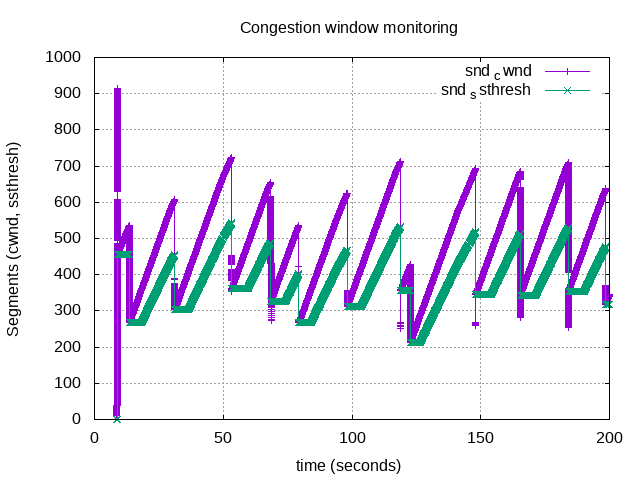
\includegraphics{lab1-group1-task2-question1.png}
	\label{fig:q21}
	\caption{T2Q1 CWND and ssthresh 0 to 200 seconds}
\end{figure}


\subsection{Q2.2 Briefly discuss the changing process.}

We see that it initally starts in slow start, until the source received three
duplicate ACKs. It then transitions to fast recovery, where it slowly increases
the congestion window until it receives a new ACK. We are now in congestion
avoidance. From there we see multiple transitions between congestion avoidance
and fast recovery, as we see the threshold halving and the CWND is adjusted to
\texttt{ssthresh + 3MSS}.


\subsection{Q2.3 Plot a graph showing CWND versus time with all the data you get.}

\begin{figure}[H]
	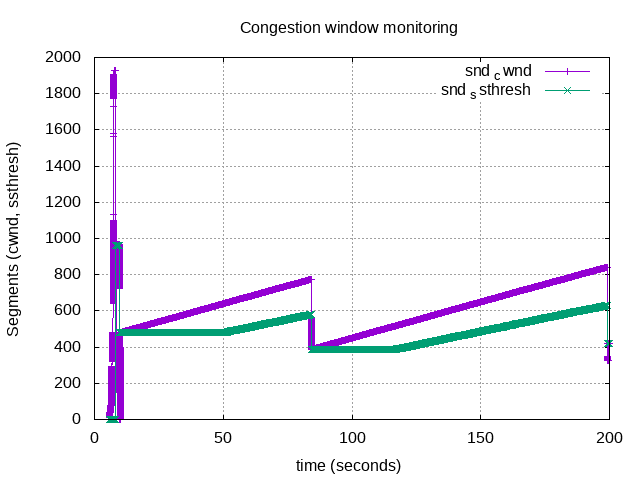
\includegraphics{lab1-group1-task2-question3.png}
	\label{fig:q23}
	\caption{T2Q3 CWND and ssthresh 0 to 200 seconds}
\end{figure}


\subsection{Q2.4 Compare this graph with the one from}

Both graphs start similarly. The relatively fast, oscillating changes between
the fast recovery and congestion avoidance states, are much slower in the
latter (figure \ref{fig:q23}). The congestion avoidance states in figure \ref{fig:q23} hold for a longer time than in figure \ref{fig:q21}. 


\subsection{Q2.5 Plot a graph showing CWND and ssthresh versus time with all the data you get.}

\begin{figure}[H]
	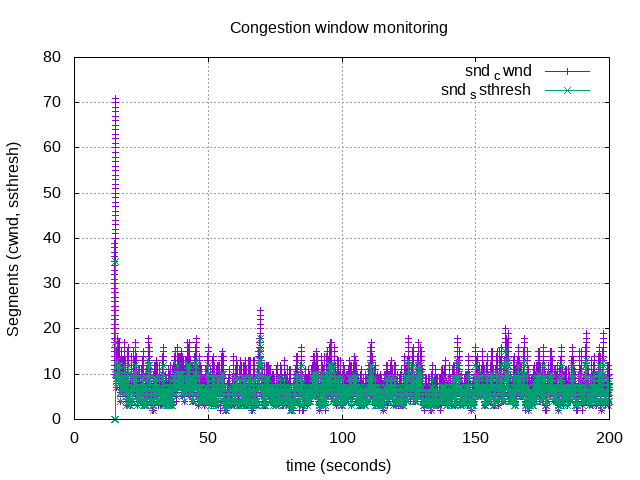
\includegraphics{lab1-group1-task2-question5.png}
	\caption{T2Q5 CWND and ssthresh 0 to 200 seconds with packet loss}
	\label{fig:q25}
\end{figure}


\subsection{Q2.6 Compare this graph with the graph of}

In this graph, the congestion window never reaches the same levels as in
previous exercises. At the peak of slow start, it is just over $70*MSS$. Here
we see a very fast oscillation between fast recovery and congestion avoidance.
It does not go back to slow start, because it never starts again with 1MSS.
This implies the throughput is much lower than in subsection \ref{sec:q21}.


\subsection{Q2.7 Zoom in the graph of this scenario (plot some parts of this scenario in a short duration, 10 or 20 seconds). Briefly explain the changing process.}

\begin{figure}[H]
	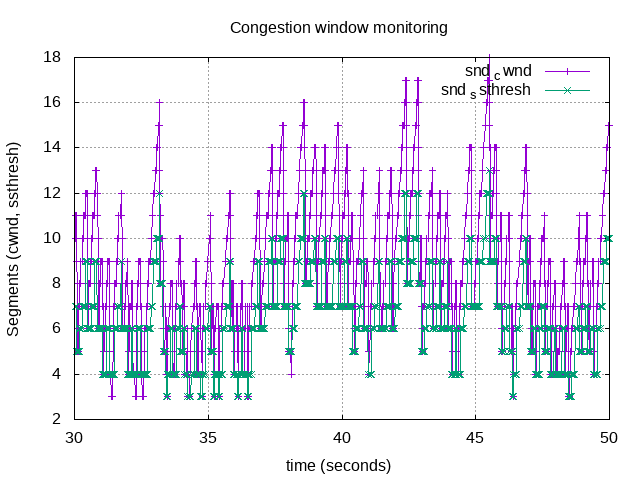
\includegraphics{lab1-group1-task2-question7-xrange-30-50.png}
	\caption{T2Q7 CWND and ssthresh 30 to 50 seconds with packet loss zoomed in}
	%\label{fig:dinges}
\end{figure}

Due to the relatively high percentage of packet loss, this connection is quite
unstable. We see the same pattern as previously, oscillating between congestion
avoidance and fast recovery, but the lowest points are as much as 8 times lower
than the peaks. Previously, the highest difference observed was around 2.8
times.


\subsection{Q2.8 Show a screen capture of the real throughput in this scenario.}

\begin{figure}[H]
	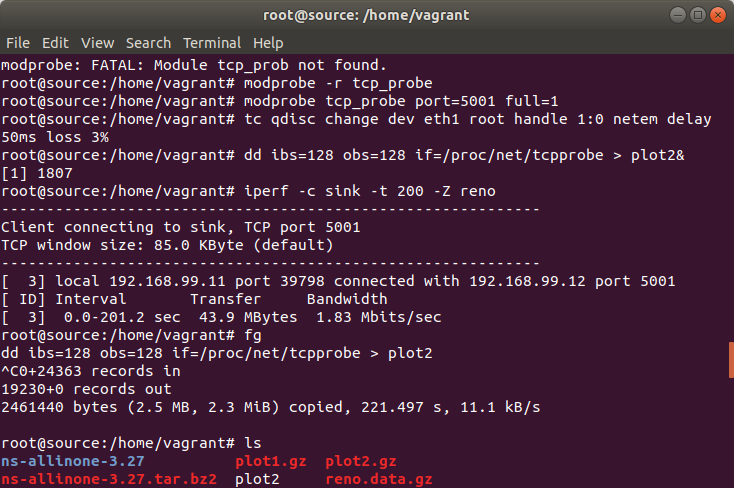
\includegraphics[width=0.8\textwidth]{lab1-group1-task2-question8.png}
	%\label{fig:dinges}
	\caption{T2Q8 Throughput of Reno algorithm}
\end{figure}


\subsection{Q2.9 Plot a graph showing CWND and ssthresh versus time with all the data you get.}

\begin{figure}[H]
	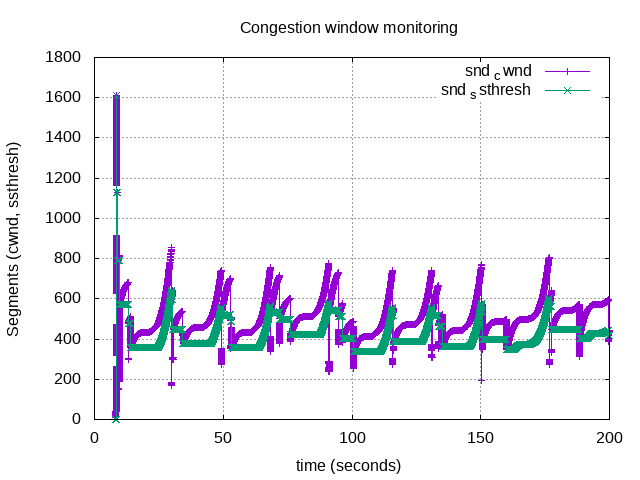
\includegraphics{lab1-group1-task2-question9.png}
	\caption{T2Q9 CWND and ssthresh 0 to 200 seconds (CUBIC)}
	%\label{fig:dinges}
\end{figure}


\subsection{Q2.10 Compare this graph with the graph of}

The main difference which catches the eye, is that it has differently-shaped,
smooth curves in the congestion window. When looking up how CUBIC works, we see
this pattern explained many times as being fast growth upon reduction on a
packet loss event, and slower probing for the maximum throughput.


\subsection{Q2.11 Plot a graph showing CWND and ssthresh versus time with all the data you get.}

\begin{figure}[H]
	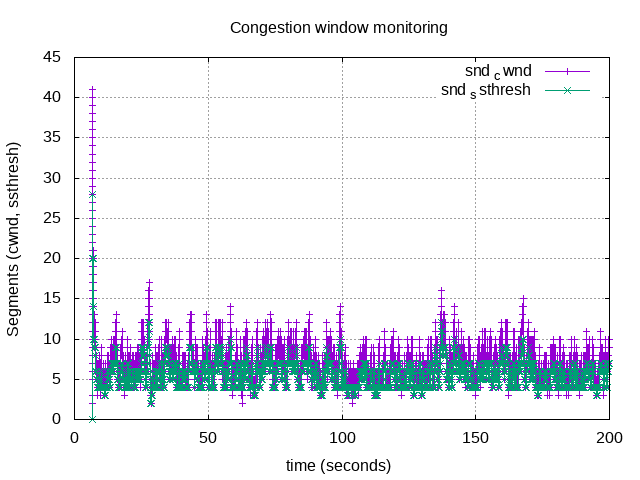
\includegraphics{lab1-group1-task2-question11.png}
	\caption{T2Q11 CWND and ssthresh 0 to 200 seconds (CUBIC) with packet loss}
	%\label{fig:dinges}
\end{figure}


\subsection{Q2.12 Compare this graph with the graph of scenario three and show the differences.}

CUBIC generally seems less aggressive. In the slow start state, it does not
reach as high as Reno ($42*MSS$ versus $71*MSS$). In the later states, it
decreases less far and usually goes down to $4*MSS$ or sometimes $3*MSS$. Reno
shows more fluctuations than CUBIC; therefore, CUBIC seems to be more stable in
those circumstances.


\subsection{Q2.13 Zoom in the graph of this scenario (plot some parts of this scenario in a short duration, 10 or 20 seconds). Briefly explain the changing process and compare it with the graph of}

\begin{figure}[H]
	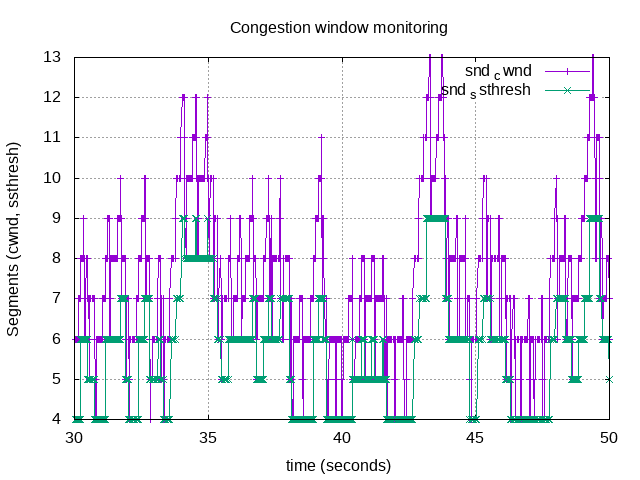
\includegraphics{lab1-group1-task2-question13-xrange-30-50.png}
	\caption{T2Q13 CWND and ssthresh 30 to 50 seconds (CUBIC) with packet loss zoomed in}
	%\label{fig:dinges}
\end{figure}

Here, too, we see that CUBIC is more stable than reno. The difference between
the minimum and maximum value, is higher in Reno. The frequency of the state
changes is also higher in Reno.


\subsection{Q2.14 Show a screen capture of the real throughput and compare it with throughput of}

\begin{figure}[H]
	%\caption{dinges}
	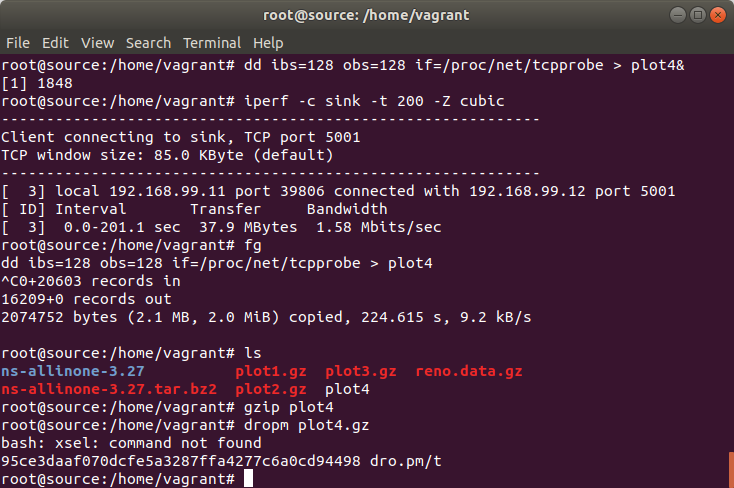
\includegraphics[width=0.8\textwidth]{lab1-group1-task2-question14.png}
	\caption{T2Q14 Throughput of CUBIC algorithm}
	%\label{fig:dinges}
\end{figure}

Reno has a higher throughput than CUBIC.


\subsection{Q3.1 Explain what an LFN network is. Change the simulation parameters to your likings and demonstrate that TcpNewReno is not suitable for LFN networks.}

An LFN (`elephant') network has a DBP (Delay-Bandwidth Product) which is
`significantly' larger than $10^{5}$ bits, i.e. multiplying the bandwidth and
the latency is larger than 12 500 bytes per second. It stands for `long, fat
network'.


\begin{figure}[H]
	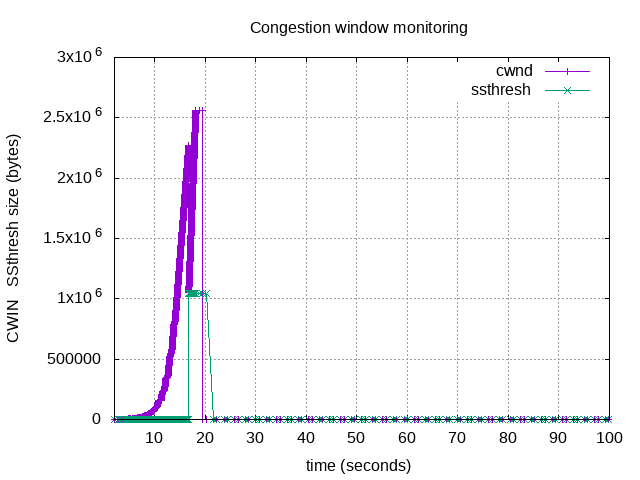
\includegraphics[width=0.8\textwidth]{lab1-group1-task3-question1-1.png}
	\caption{T3Q1 LFN Enabled on TCPNewReno 0 to 100 seconds}
	\label{fig:q311}
\end{figure}


\begin{figure}[H]
	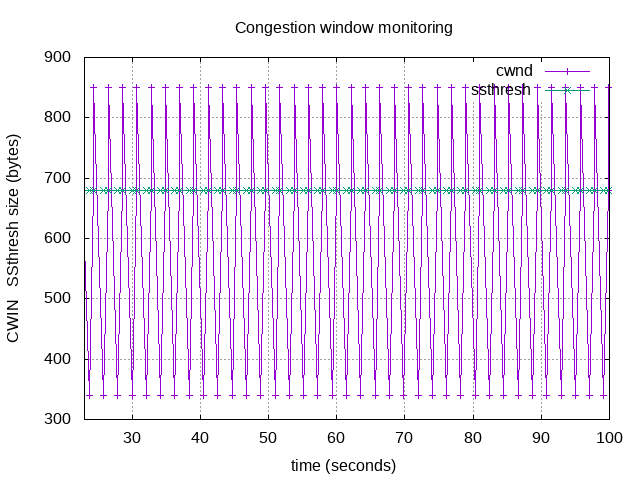
\includegraphics[width=0.8\textwidth]{lab1-group1-task3-question1-2.png}
	\caption{T3Q1 LFN Enabled on TCPNewReno 23 to 100 seconds}
	\label{fig:q312}
\end{figure}

Figure \ref{fig:q311} shows a long slow start and congestion avoidance phase of approximately 20 seconds, which is followed by a low throughput. This is depicted in figure \ref{fig:q312}.
We configured the network to have a throughput of 500 Mbps and a delay of 300ms. We see that TCPNewReno does not reach 500 Mbps by far. Therefore TCPNewReno is not suitable for LFN networks.

\subsection{Q3.2 Explain SACK does. Change the simulation parameters to your likings and demonstrate the performance improvement with SACK.}

Defined in RFC 2018, SACK allows receivers to indicate they have received segments which are not contiguous.

\begin{figure}[H]
	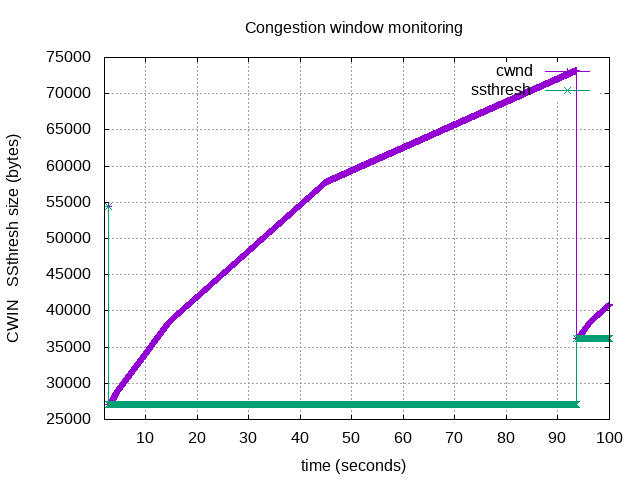
\includegraphics[width=0.8\textwidth]{lab1-group1-task3-question2.png}
	\caption{T3Q2 SACK Enabled on TCPNewReno}
	\label{fig:q32}
\end{figure}

According to figure \ref{fig:q32} higher bandwidths are reached and fewer fluctuations are shown during the simulation, compared to the previous experiments without SACK enabled.


\subsection{Q3.3 Explain with TCP fairness is. Show the effect of multiple flows in the simulation.}

As described by Gorp and Gommans\cite{gg}:

\begin{quote}
	,,In datacenters, multiple tenants share a finite amount of bandwidth. When an uplink
	is saturated, packets that overflow available buffer space will be dropped and have to
	be retransmitted by the sender. When one tenant chooses to retransmit faster than
	others, they have an advantage as they will make it though more quickly. TCP is
	a connection-oriented protocol which employs congestion control algorithms. These
	algorithms aim to divide the available bandwidth equally between network flows.

	Some congestion control algorithms are more aggressive than others, and it has been
	reported that some algorithms cause others to back off excessively. Tenants may,
	perhaps inadvertently, cause unequal bandwidth distributions during times of congestion.''
\end{quote}

While no case was found of unfairness, other than Microsoft Windows' CTCP (but
that behaviour was so strange that its test was labeled inconclusive), some
have much better performance in specific scenarios. In figure
\ref{fig:cubic-bic-8-12}, CUBIC and BIC are shown to perform comparatively in
high loss conditions. In figure \ref{fig:cubic-bbr-8-12}, the same situation is
shown but with CUBIC and BBR. In figure \ref{fig:cubic-bic-8-0}, CUBIC is
compared with BIC with 8ms delay and 0\% loss. It is shown that the algorithms
perform equally and allocate an amount of bandwidth so equal that on this
scale, no difference is visible at all during the majority of the test. Any
difference visible, is attributed to random variance.

\begin{figure}[H]
	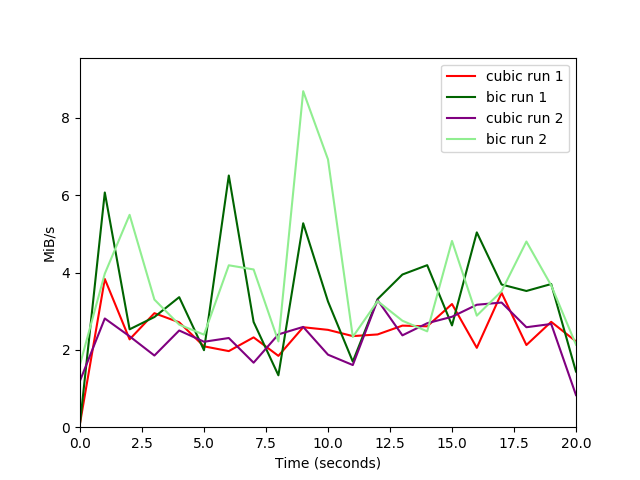
\includegraphics{cubic_vs_bic_8_12.png}
	\caption{CUBIC vs. BIC, 8ms delay, 1.2\% loss}
	\label{fig:cubic-bic-8-12}
\end{figure}

\begin{figure}[H]
	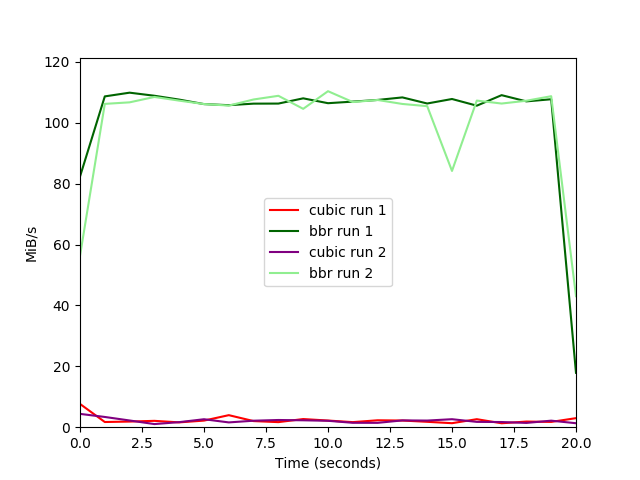
\includegraphics{cubic_vs_bbr_8_12.png}
	\caption{CUBIC vs. BBR, 8ms delay, 1.2\% loss}
	\label{fig:cubic-bbr-8-12}
\end{figure}

\begin{figure}[H]
	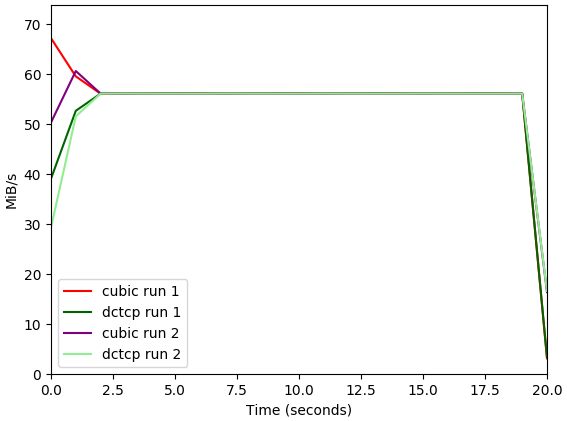
\includegraphics[width=\textwidth]{cubic-bic-8-0.png}
	\caption{CUBIC vs. BIC, 8ms delay, 0\% loss}
	\label{fig:cubic-bic-8-0}
\end{figure}


\subsection{Q3.4 Replicate scenario 3 of the emulation: packet loss of 3\%, delay of 50 ms and transfer duration of 200sec. Use TcpNewReno. Compare the two results.}
The plot from \texttt{ns3} is shown in figure \ref{fig:q34}.

\begin{figure}[H]
	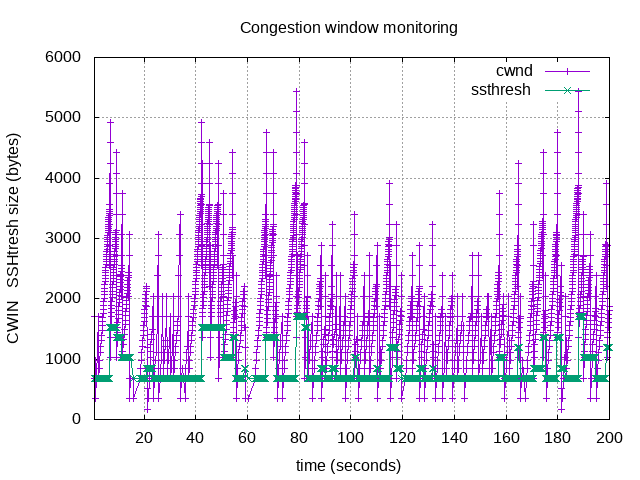
\includegraphics{lab1-group1-task3-question4.png}
	\caption{CWND and ssthresh 0 to 200 seconds for TCPNewReno with packet loss and delay}
	\label{fig:q34}
\end{figure}

The results in ns3 compared to scenario 3 show different data. Figure \ref{fig:q34} shows the size in bytes of $cwnd$ and $ssthresh$, while figure \ref{fig:q25}
shows the amount of segments. The amount of segments sent according to figure \ref{fig:q25} fluctuates more than the size of $cwnd$ in bytes. The default MTU in ns3 is 400 bytes.
We see that it subtracts the IP-header, TCP-header and 20 bytes resulting in an MSS of 340 bytes. If we divide the window sizes at multiple points in figure \ref{fig:q34} by
340 bytes, the resulting amount of segments corresponds to the amount of segments from figure \ref{fig:q25}. This is however, not exactly checked due to the density of figure \ref{fig:q25}.


\subsection{Q3.5 After these experiments, please briefly describe the difference between simulation and emulation?}

\begin{quote}
,,Emulation is the process of mimicking the outwardly observable behavior to
match an existing target. The internal state of the emulation mechanism does
not have to accurately reflect the internal state of the target which it is
emulating.

Simulation, on the other hand, involves modeling the underlying state of the
target. The end result of a good simulation is that the simulation model will
emulate the target which it is simulating.''
\end{quote}

From Toybuilder on StackOverflow\cite{toybuilder}.

In our case, the emulator is NS3 and the simulation is done using iperf.


\printbibliography

\end{document}
